\section{Relational Web Management
	Platform}\label{relational-web-management-platform}

Written by Paul Wille

We decided to have a separate system component to manage the metadata of
data-sources that shall be imported and that already have been or are
ongoingly imported. This system shall fulfill several tasks that are
important for organizing the importing/ETL-process. Furthermore it
provides imortant information to several other system components.

In this chapter we will discuss why we decided to include such a system,
what it was build for and how we achieved this.

\subsection{Purpose of the System}\label{purpose-of-the-system}

This main purposes of the system are:

\begin{itemize}
	\item
	The user registering and describing a datasources that is going to be
	imported
	\item
	Providing this metadata information regarding the datasources to other
	system-components
	\item
	Provide users that want to import data with information about units
	\item
	Enabling visitors or users, that want to use the data that exists (and
	not import new data), to see the listed resources our system contains
\end{itemize}



\subsubsection{Registering Sources}\label{registering-sources}

\paragraph{}
To each datasource there is important information and metadata that must
be known to our system before importing the datasource. This information

\begin{itemize}
	\item
	must be known upfront
	\item
	does only contain metainformation about the sources
	\item
	has no direct relation to actual measurement-data
	\item
	is quite static and does not change over time.
\end{itemize}

Therefore we chose not to manage it in the same database as the saved
extracted and transformed datapoints of the sensor-data-sources, but
have a separate system. With this we can tweak the data-storage
component for providing and fullfilling its main tasks and do not mix up
meta-information and actual sensordata in one place.

Meta-Information that has to be provided to our system prior to
importing for several reasons are mainly:

\begin{itemize}
	\item
	Name of source
	\item
	The startdate, from which on the source provides data
	\item
	if the source is still active (data is being appended to the source in
	the future).
	\item
	If not so: the end date of measurements
	\item
	Under what license the data is published
\end{itemize}

Additionally we ask the user to give additional information, that is
useful for our system

\begin{itemize}
	\item
	If the datasource is still active: At what schedule is new data
	published
	\item
	A \emph{slug} that can be used as an id within our pipeline and in
	ElasticSearch
	\item
	Which measurements the data source provides (which actual measurements
	the data-source collects)
	\item
	The location of the docker container as URL
\end{itemize}

\begin{figure}
	\begin{center}
		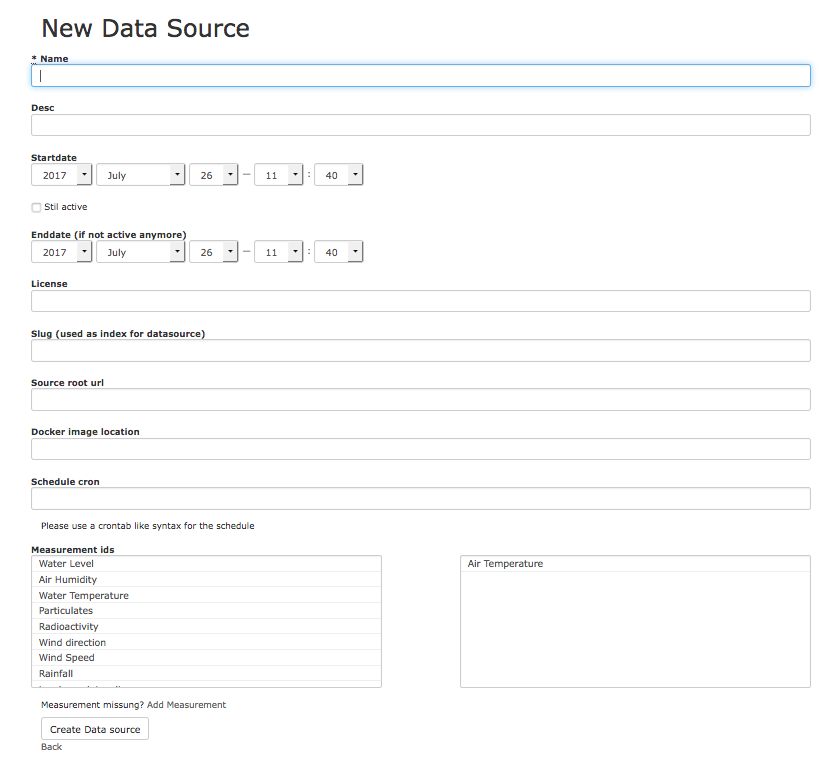
\includegraphics[width=0.7\textwidth]{08_web_mgmt/images/new_datasource.png}
		\caption{Registering a data source within the Web management platform.}
		\label{image_new_source}
	\end{center}
\end{figure}

\subsubsection{Provide information to other system-components}

\paragraph{Provide Validation Schema}\label{provide-validation-schema}

\paragraph{}
As described in the chapter about validation and inserting to
ElasticSearch we have a distinct component, seperated from the
importers, that will handle the validation of the outcome of those. This
schema has to be provided. The actual schema itself is fixed and could
be hardcoded to the validator, without need to make another
http-request.

Because of two reasons we decided that this would be a bad idea:

\begin{itemize}
	\item
	In order to validate that datasource-dependent information in the
	outcome is correct as well, there are dynamic contents within the
	validation schema (mostly the id of the data source to prevent
	insertion with the wrong id)
	\item
	If the schema changes over time, correcting information hardcoded
	within the validator would need a complete redeploy and change of the
	validator as such
\end{itemize}

Therefore we needed a place where said validation-schema can reside. The
web management system seemed to be the right pace for that, as it caries
metainformation about datasources anyways and the datasources are
registered there. So it is easy to provide the relevant information
aswell. The management system provides an api call to supply the
validation schema to the validators that looks like this:

\begin{verbatim}
GET /data_sources/:id/getValidationSchema
\end{verbatim}

The Response looks like this. The const \texttt{source\_id} thereby will
be replaced by the ID of the data source

\begin{verbatim}
{
	"$schema": "http://json-schema.org/schema#",
	"title": "Data Source",
	"description": "A Data Source for Open Sensor Data from the CP project at TU Berlin. ",
	"type": "object",
	"properties": {
		"source_id": {"const": "source_slug"},
		"device": {"type": "string"},
		"timestamp": { "type": "string", "format": "date-time" },
		"timestamp_data": { "type": "string", "format": "date-time" },
		"location": {
			"type": "object",
			"properties": {
				"lat": {
					"type": "number",
					"exclusiveMaximum": true,
					"exclusiveMinimum": true,
					"maximum": 90,
					"minimum": -90
				},
				"lon": {
					"type": "number",
					"exclusiveMaximum": true,
					"exclusiveMinimum": true,
					"maximum": 180,
					"minimum": -180,
				}
			},
			"required": ["lat", "lon"]
		},
		"license": {"type": "string"},
		"sensors": {
			"type": "object",
			"items": [
				{
				"type": "object",
				"properties": {
					"sensor": {"type": "string"},
					"observation_type": {"type": "string"},
					"observation_value": {"type": "number"}
				}
			}]
		}
	},
	"required": ["source_id", "timestamp","sensors", "location", "license"]
}
\end{verbatim}

\paragraph{Provide Information to Elastic Search API for query
	optimization}\label{provide-information-to-elastic-search-api-for-query-optimization}

\paragraph{}
Like desdcribed in the section about our data model and Elasticsearch as
a data-storage-component our data-model is datasource-based and not
measurement based. For certain types of queries that tackle measurements
it will though be important to have further information on the
connection between data sources and measurements.

As there where several possibilities where this information could be
stored and managed and how it would be provided, the easiest to start
with was in our opinion, that the implementer of an importer provides
this information to us, when registering his datasource. The user
therefore has to mark what measurements a datasource contains upfront (See Figure \ref{image_new_source}).

In order to optimize querying our data this information is provided to
the API that wraps the search interface of Elasticsearch via an API
itself. The information is stored in an indexed join table that holds
this n-to-n mapping between measurements and datasources. As you can see
in the class diagram (See Figure \ref{image_uml_webmgmt}) of the relational system,
queries in both directions are provided: getting all measurements, a
datasource provides and getting all datasources that contain a given
measurement. The corresponding rout es look like this:

\begin{verbatim}
GET /data_sources/:id/measurements
\end{verbatim}

An example request would look like following:

\begin{verbatim}
GET /data_sources/blume_messnetz/measurements

[
	{
		"id":1,
		"name":"Air Temperature",
		"desc":"",
		"unit_category_id":"temperature"
	},
	{
		"id":3,
		"name":"Air Humidity",
		"desc":"amount of water vapor present in the air",
		"unit_category_id":"humidity"
	}
]
\end{verbatim}

\begin{verbatim}
GET /measurements/:id/data_sources
\end{verbatim}

An example request would look like following

\begin{verbatim}
GET /measurements/1/data_sources

[
	{"id":1,"slug":"blume_messnetz","license":""},
	{"id":5,"slug":"german_weather_service","license":""}
]
\end{verbatim}

\paragraph{Provide configuration information to the
	importer-deployment-component}\label{provide-configuration-information-to-the-importer-deployment-component}

As the registering should be at best the only step, in which the
implementer has to provide information to our system besides providing
the importer itself it should preferably cover all information needed to
get an importer running.

\subsection{Requirements}\label{requirements}

In contrast to nearly every other system component we had to build, the
management platform had to meet not as many criteria that one would
expect from a distributed cloud-system in general. Most of the data the
system will contain is quite static data and the number of requests that
we expect is also quite low.

\begin{itemize}
	\item
	Availability to other system components, that require the held
	information
	\item
	Quick response time (for qury-optimization within the public
	search-API)
	\item
	Ability to run asynchronous background tasks (for scheduling)
\end{itemize}

While those requirements look like those of a cloud-system, taking a
closer look exposed, that a good caching solution would be sufficient in
our case. If the system would grow bigger it would stil require to be
scaled in some way. But as the information in the managament database
will change very slowly we decided, that this could be achieved by
prepending a distributed caching system, like for example using
\emph{Redis} for that. By that we would achieve quick response times and
availability, as \emph{Redis} can be distributed and read accesses are
very fast and possible on all nodes. Writing is quite expensive due to
the replication method used by Redis but it would be sufficient to updte
the cache several times a day with new information from the
management-database, so we considered this a shortfall, we could take.

\subsection{Architectural Details}\label{architectural-details}

The system was built using \emph{RubyOnRails} with \emph{PostgreSQL} as
a database. The reasons why we chose to use RubyOnRails are:

\begin{itemize}
	\item
	Relatively fast developement of an MVC-Web-application
	\item
	RoR is established for over a decade, has therefore lots of resources
	- also for all kinds of extensions
	\item
	Extensive community support
	\item
	Very good integrated ORM adapters, that could easily be exchanged for
	e.g.~ODM adapters for e.g.~mongodb
	\item
	Offers the dynamic of Ruby as programming language
\end{itemize}

As mentioned before, the planning of the extent of the functionalitly
offered by this system, was very vague. Besides managing metadata and
providing an API for other components, further features were at least
considered to be part of this system, like for example a scheduler that
triggers the component that handles the deploy of importers. Therefore
we chose to build this system on top of an infrastructure, that can be
easily extended in many directions and has nice to use database adapters
instead of a more lightweight system.

While initially we also wanted to model a data source with its sensors
grouped in sensor stations, this approach would bring imense overhead
for configuring datasources in our system upfront, as a user would have
to very exactly model a data source with all its sensors and sensor
stations first. For big services like e.g.~the German Weather Servide
this would be an enormous amount of work. Gathering this information
would better be done by scraping the information present in
Elasticsearch and translating them to geolocated information for all
sensors/sensor-stations/datasources. In Figure \ref{image_uml_webmgmt} you can
see the modeling for this approach greyed out.

The main metainformation about the datasources (besides metadata about
the source itself) that we still needed within our system (the locality
of the sensor and the grouping of sensor stations is not essential for
our system to work) and had to offer to the user registering a source
were then:

\begin{itemize}
	\item
	Information about the measurements a datasource offers data for
	\item
	Information what unit we use for a measurement as main unit (see
	section Unit system // TODO ref section)
\end{itemize}

\begin{figure}
	\begin{center}
		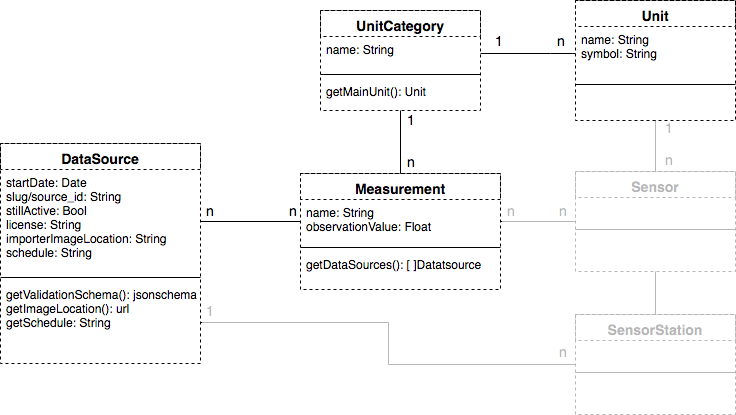
\includegraphics[width=0.9\textwidth]{08_web_mgmt/images/relational_schema.png}
		\caption{UML Class-Diagram of the Relational Management System. The greyed out parts are showed for informational reasons and are not used anymore.}
		\label{image_uml_webmgmt}
	\end{center}
\end{figure}



\subsubsection{Future Improvements}\label{future-improvements}

\paragraph{Exchange Scheduling
	information}\label{exchange-scheduling-information}

Due to not reaching every goal of our initial plan on how the
architecture should look like, the scheduler had to move to the
component managing the deploy on a Kubernetes cluster. While this
component should be resposible for deploying importers for a datasource
aswell in the future, the information about the schedule should actually
be provided to the web management system by the user. This is currently
not happening. There would be several ways how to manage scheduling
and/or deliver the scheduling information from this system to the
component handling the scheduling.

\begin{itemize}
	\item
	Having a background-processing component that acts as a scheduler
	withing the web management platform. This would require an API to
	trigger the deploy on the component responsible for that, which we
	were not able to achieve.
	\item
	Having a microservice-like component, that is only responsible for
	scheduling and triggering importers to be deployed. This would aswell
	require an API on the deploying-component.
	\item
	Leaving the scheduling within the deploying-component. This would also
	require an API in it, but just for receiving the genereal schedule,
	not for offering a hook to trigger an import.
\end{itemize}

The second option seems more granular and more conform to our general
microservice-approach but would also require the most configuration and
deployment effort. Including a scheduler in the web management platform
would somehow violate this approach but still make sense, as this
component could easily be integrated within RubyOnRails and would be a
standalone component within it.

\paragraph{Caching}\label{caching}

There is currently no caching-solution, as the workloads during the
developement phase were quite manageable Also including a distributed
caching system in our production pipeline seemed to be too high effort
and would take up many resources, that would actually not be needed.
Therefore we wanted to use the limeted and expensive resources we had
for actual importing. Extending the System itself to use caching with
Redis would be very easy achievable though.

\subsection{Unit System}\label{unit-system}

When it comes to gather and manage sensor data one topic that directly
comes to mind is that of units. Uncountable units exist and while there
are international systems like the \emph{International System of Units
	(SI)} or the \emph{metric system} it is hard to find one system, that
fits all possible measurements in our case. Some of the reasons for that
are:

\begin{itemize}
	\item
	Not for all measurements there exists an standardized unit in unit
	systems (e.g.~parts per million)
	\item
	While standardized systems have the advantage of offering \emph{one}
	standard unit for a category, those do not have to be intuitive
	(e.g.~using Kelvin for outside temperature probably will not be
	intuitive for many people)
\end{itemize}

Because of that we had to think of an own way, how units would be
chosen, managed and how users would get information about them.

\subsubsection{Further requirements}\label{further-requirements}

\paragraph{}
Deciding on a strategy to model units, was a quite long process and not
all requirements could be fullfilled. In this section we will discuss
the most important requirements to later on explain for what approach we

\begin{enumerate}
	\def\labelenumi{\arabic{enumi}.}
	\item
	Allow convertability and ability to localize
	\item
	It has to be understandable, in what unit a measurement is expressed
	and in which it was measured It is absolutely avoidable that
	measurements exist in the database, with a not understandable unit or
	even worse with a unit that differs from what the system supposes the
	measurement is expressed in. It is therefore advisable to enfoce the
	user to handle units carefully
	\item
	Each unit should only exist once. Typos, different exprsssions etc.
	shall not lead to confusion
\end{enumerate}

\subsubsection{Implementation}\label{implementation}

\paragraph{}
With the requirements in mind we decided to organize units like so:

\begin{enumerate}
	\def\labelenumi{\arabic{enumi}.}
	\item
	We introduced \textbf{Unit Categories}. Units themselves always belong
	to a unit category. The unit-category desribes an entity for which
	measurements exist, which express their observations with one of the
	units of that category (See Figure \ref{image_uml_webmgmt} for Class Diagram ).
	\item
	Each unit has a \textbf{main unit} that we decide on. By calling the
	api or visiting the management platform a user can see, which the main
	unit is. Within our datastore we only use the main unit of a
	unit-category for expressing measurements.
	\item
	Units are managed by admins repectively users with permit to do so.
	\item
	We therefore have a curated list of the unit-categories and units
	\item
	If there are units, measurements or even categories missing, each user
	can propose new ones. This proposals are also managed by the group of
	people managing the units.
\end{enumerate}

Measurements are controlled on the platform itself to allow users to
better propose new measurements, as this may happen more often. Units
and the Unit categories however are managed in a \emph{.yml} file. The
syntax we used looks like following for one entry:

\begin{verbatim}
From config/constants/units.yml:

pascal:
	id: pressure_pascal
	name: "pascal"
	unit_symbol: "pa"
	unit_category_id: pressure
	notation: "1 <centerdot>
				<mfrac>
					<mrow>
						kg
					</mrow>
					<mrow>
						m 
						<msup>
						<mi>s</mi>
						<mn>2</mn>
					</mrow>
				</mfrac>"

From config/constants/unit_categories.yml:

pressure:
	id: pressure
	name: Pressure
\end{verbatim}

The unit categories are pretty straight forward. For a unit there are
some more possibilities. Besides declaring the unit symbol, the category
it belongs to, its name you are allowed to use MathML to express what
the meaning of a unit is. This is especially helpful with units that can
be directly converted to each other (See Figure \ref{image_unit}).


\begin{figure}
	\begin{center}
		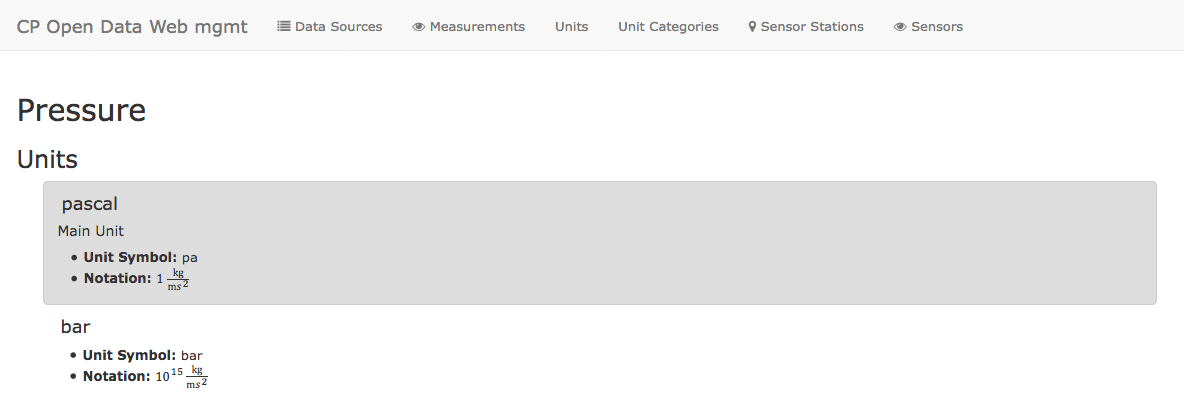
\includegraphics[width=0.7\textwidth]{08_web_mgmt/images/unit_frontend.png}
		\caption{Screenshot of the units of a unit category on the web
			management platform. You can see the main unit and have a notation on
			what the units express.}
		\label{image_unit}
	\end{center}
\end{figure}



The API of the web management system also provides calls to a) receive
the main unit of a unit category and to b) get a list of all units there
are for a unit category. Both of these information are of course aswell
accessible from the frontend of the system.

\begin{verbatim}
GET /unit_categories/:id/getMainUnit
\end{verbatim}

Example request:

\begin{verbatim}
GET /unit_categories/temperature/getMainUnit

{
	"id":"temperature_celsius",
	"name":"celsius",
	"unit_category_id":"temperature",
	"unit_symbol":"°C"
}
\end{verbatim}

\begin{verbatim}
GET /unit_categories/:id/units
\end{verbatim}

Example request:

\begin{verbatim}
GET /unit_categories/temperature/units

[
	{"attributes":
		{
			"id":"temperature_celsius",
			"name":"celsius",
			"unit_symbol":"°C",
			"unit_category_id":"temperature",
			"notation":""
		}
	},
	{"attributes":
		{
			"id":"temperature_fahrenheit",
			"name":"fahrenheit",
			"unit_symbol":"°F",
			"unit_category_id":"temperature",
			"notation":""}
	},
	{"attributes":
		{
			"id":"temperature_kelvin",
			"name":"kelvin",
			"unit_symbol":"K",
			"unit_category_id":"temperature",
			"notation":""
		}
	}
	[...]
]
\end{verbatim}

\subsubsection{Discussion of our approach}\label{discussion-of-our-approach}

\paragraph{}

This implementation has some advantages but also some disadvantages. In
this section we want to take a closer look to both sides.

As we force the user to use our main unit, we can be sure, that all data
in the database is of the same unit for a measurent type. Of course we
cannot enforce, that the user does convert his measurements or does it
right, but this counts as a faulty import, which is the responsibility
of the user anyways. Of course an assessment if data is legit would be
nice, but this is also hard to achieve and not in the scope of our
project.

Our approach of having a curated list of course means some management
overhead and possible waittimes for the user, if something is not
present yet. But to us this seemed like the only way in order to prevent
doublings of units/measurements etc. and a chaos with the unis.

As the unit categories should be present after a short testing phase of
a system, and a main unit exists with with, as the curators decide on
one, the user should most of the time be able to register a source, when
he wants to, as he only needs to know the main unit.

A big advantage of our approach is, that we kind of crowd-source the
implementation of converters by this, as it happens during the ETL phase
while importing (See //TODO ref chapter unit conversion) a source. This
gives us a chance to achieve the following:

\begin{itemize}
	\item
	Conversions can be retraced, as it is known, which converter a user
	used
	\item
	Localization within our database can easily be done, as all
	measurements of a unit category have the same unit and converters are
	written the moment someone has to convert his source data to our
	preferred unit.
	\item
	By corwd-sourcing the implementation of converteres they are also open
	sourced for reuse by other users. Having our own converters only in
	the system to convert measurements after they are in the database
	would not guarantee the reusability as importers and our database
	frontend depend on totally different things.
\end{itemize}
